\documentclass[../notes.tex]{subfiles}

\pagestyle{main}
\renewcommand{\chaptermark}[1]{\markboth{\chaptername\ \thechapter\ (#1)}{}}
\setcounter{chapter}{2}

\begin{document}




\chapter{Condensations}
\section{Problems 1, 4, and 8}
\begin{itemize}
    \item \marginnote{9/16:}David works with Rick Danheiser.
    \item We now begin discussing Problem 1.
    \begin{figure}[h!]
        \centering
        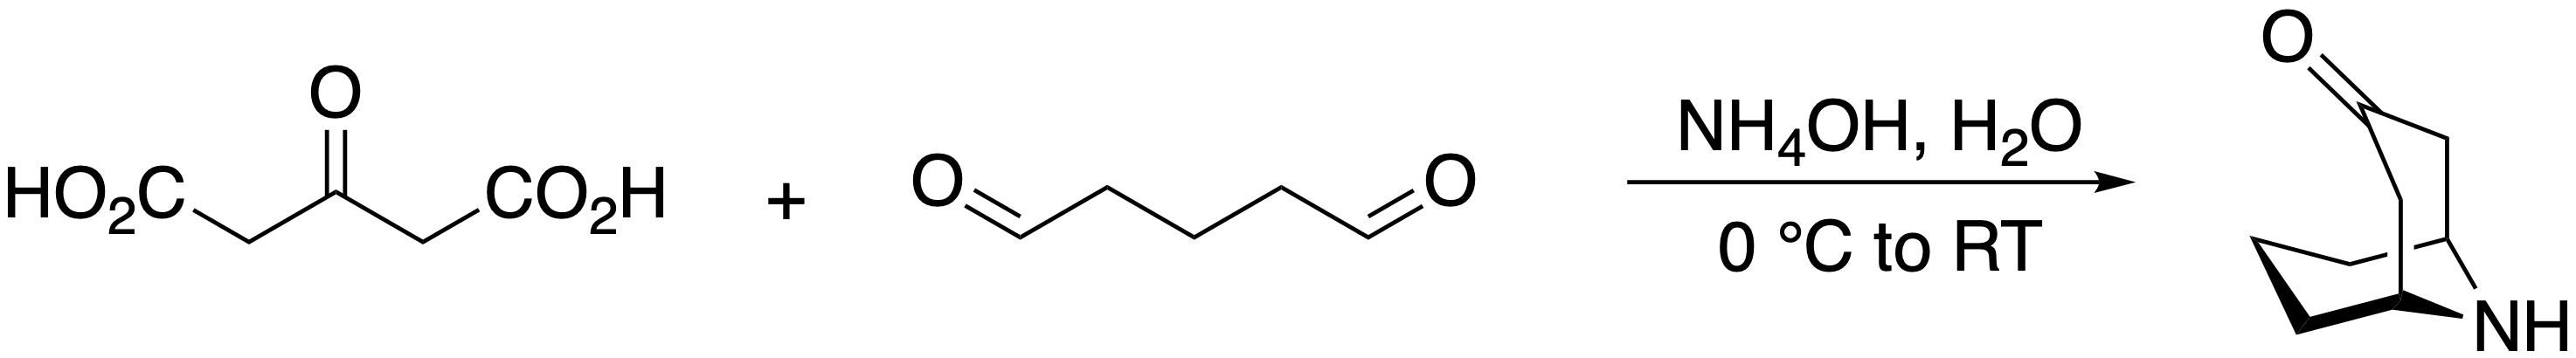
\includegraphics[width=0.6\linewidth]{WPSet1Q1.png}
        \caption{Wendlandt PSet 1, Q1.}
        \label{fig:WPSet1Q1}
    \end{figure}
    \item The reagents: \ce{NH4OH} in water is approximately $\pH=11$.
    \item Keto-enol tautomerization and amine condensation gets the carbons bonded in the right way.
    \begin{itemize}
        \item Dialdehyde forms an imine.
        \item The enol is not unreasonable because hydrogen bonding stabilizes a 6-membered ring.
        \item Then the enol can be a H-bond acceptor from the other carboxylate.
    \end{itemize}
    \item Watch out for reversible steps!!
    \item Loss of \ce{CO2} helps drive some of the steps.
    \item There are multiple right answers; David's sequence of events works, but others could be valid, too.
    \item Aldehyde is more electrophilic than the monoprotonated imine, so if we're gonna react with an imine, we need to change both aldehydes into imines first. Alternatively, we need to diprotonate the imine.
    \item It's not clear whether decarboxylation happens earlier or later in the mechanism.
    \item Altogether, the full solution to PSet 1, Q1 is on the next page.
    \begin{figure}[H]
        \centering
        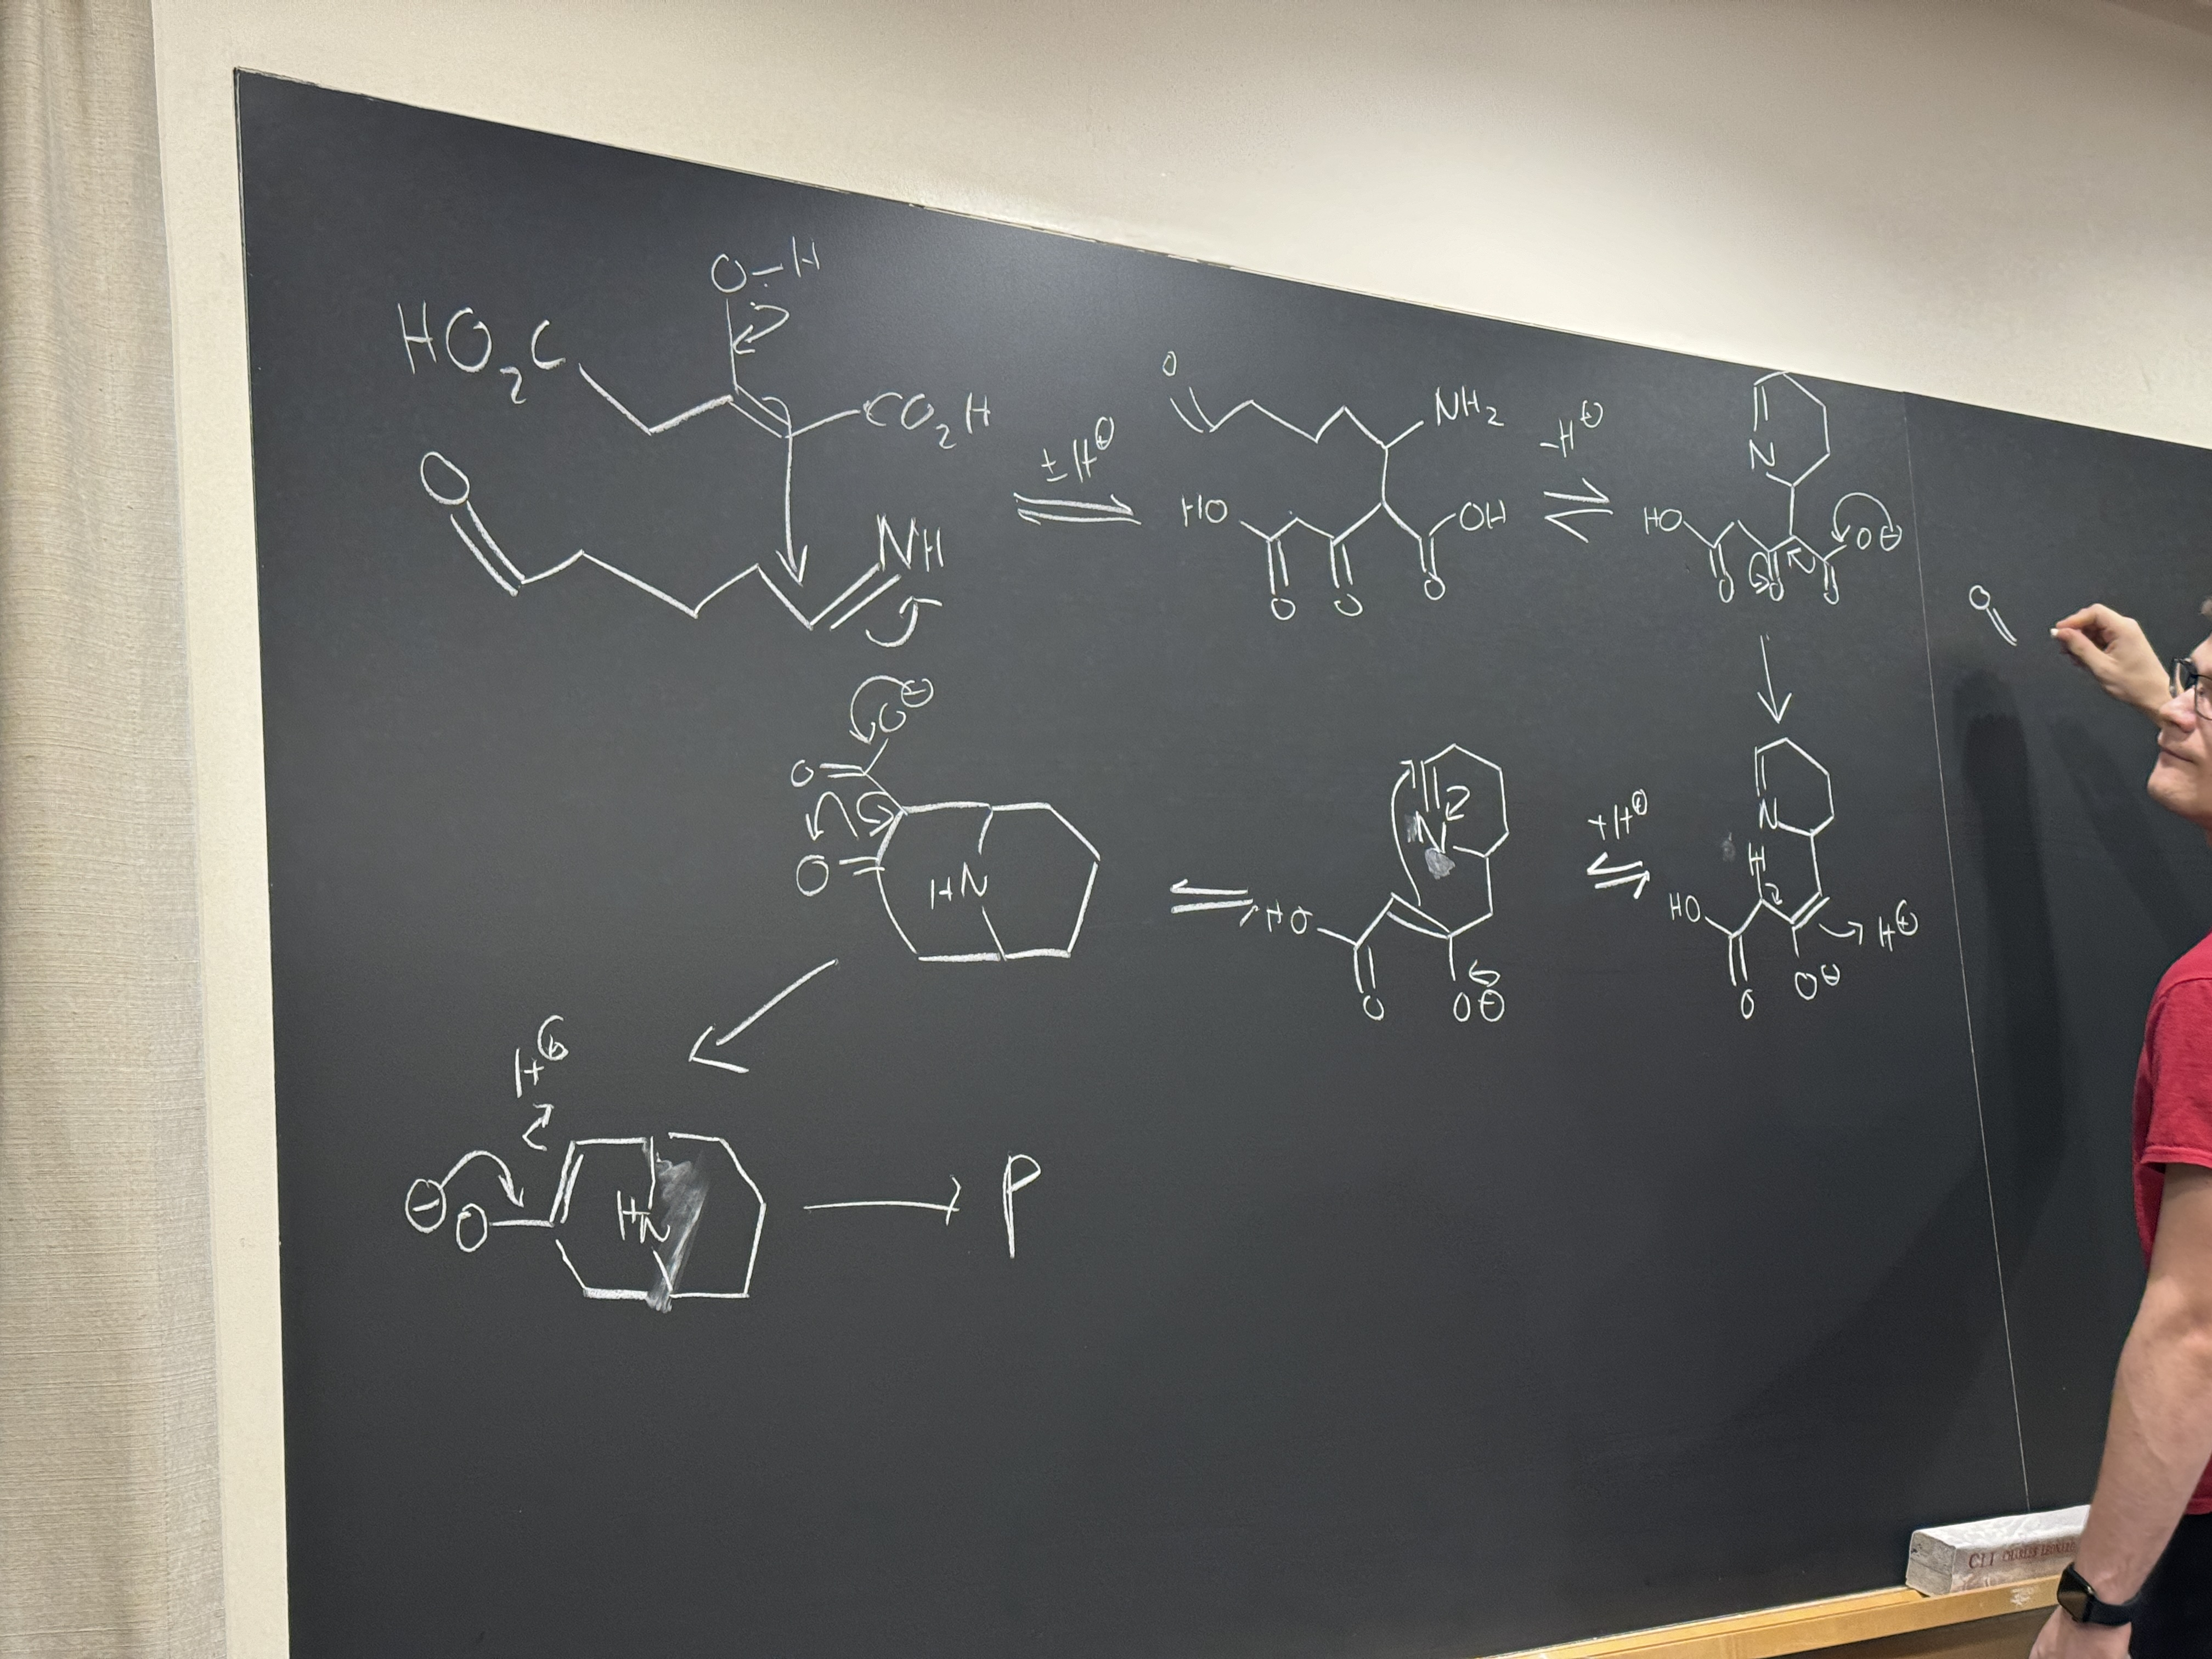
\includegraphics[width=0.8\linewidth]{WPSet1Q1S.JPG}
        \caption{Wendlandt PSet 1, Q1 solution.}
        \label{fig:WPSet1Q1S}
    \end{figure}
    \pagebreak
    \item We now begin discussing Problem 4.
    \begin{figure}[h!]
        \centering
        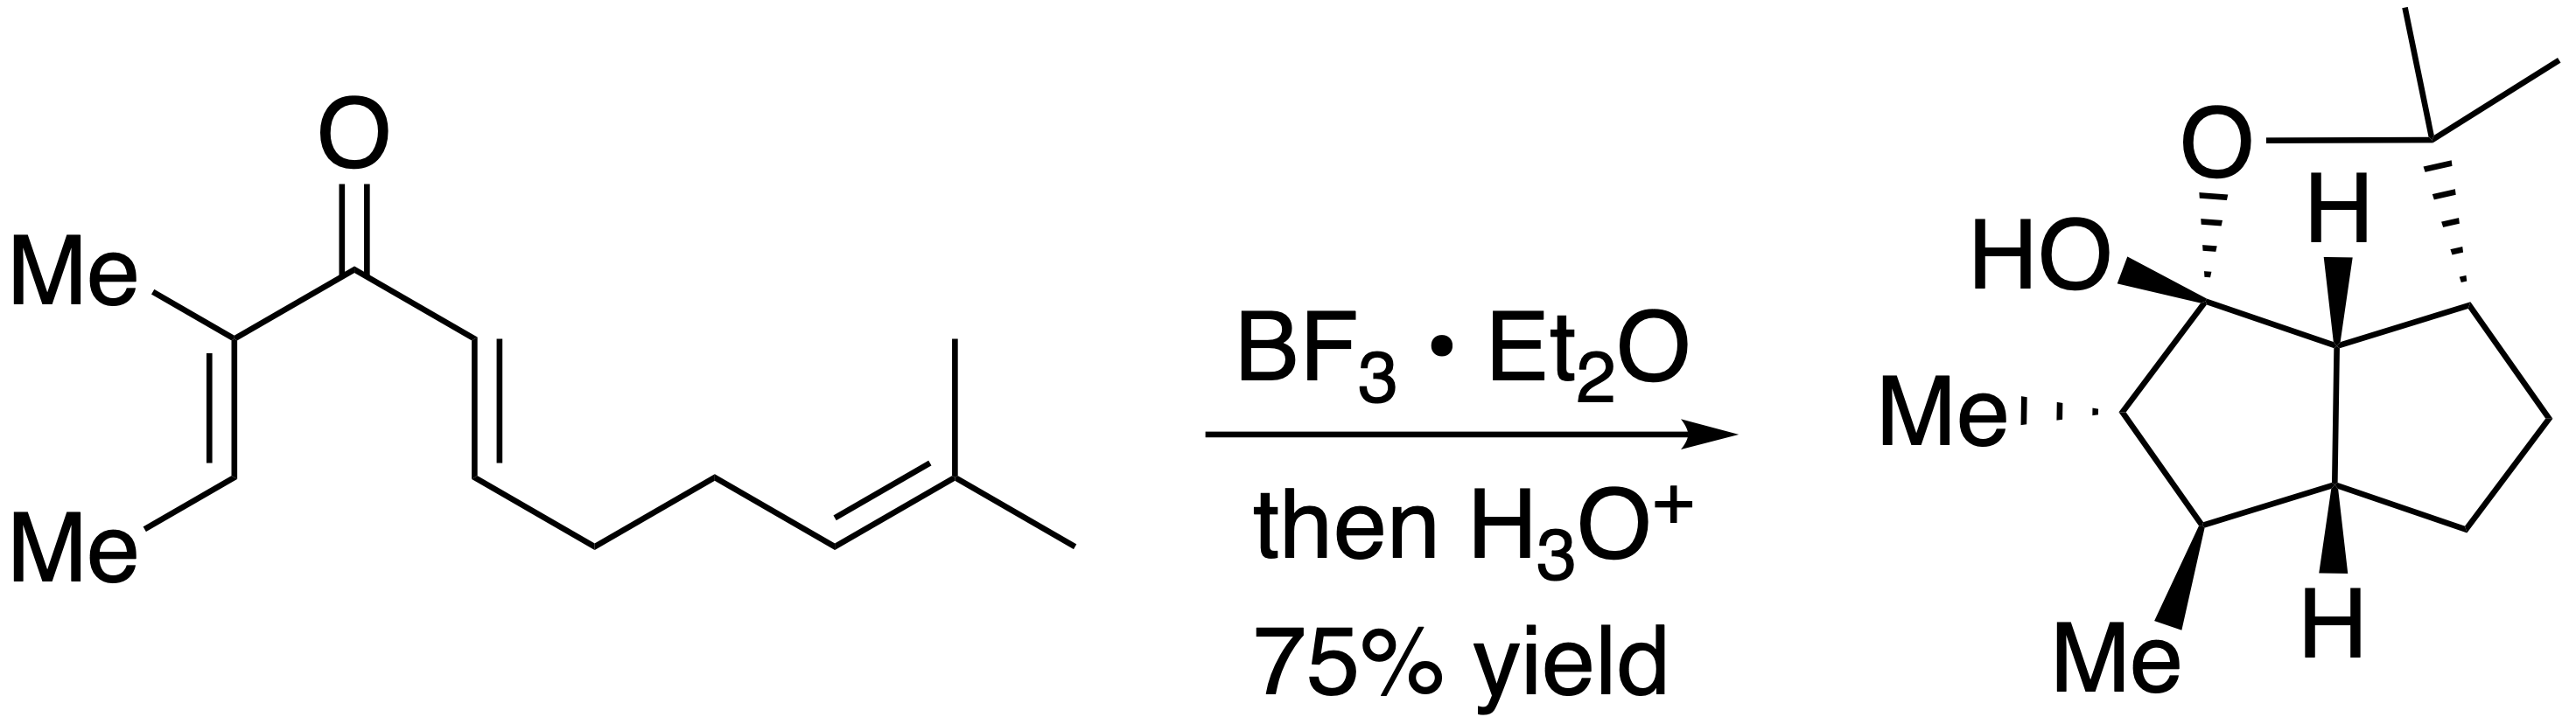
\includegraphics[width=0.45\linewidth]{WPSet1Q4.png}
        \caption{Wendlandt PSet 1, Q4.}
        \label{fig:WPSet1Q4}
    \end{figure}
    \item This is a \textbf{Nazarov reaction}, which is covered in Clayden.
    \item The initial electrocyclization is conrotatory; we need a continuous sequence of $\pi$-orbitals to get this.
    \item The Nazarov is a very powerful tool for making 5-membered rings, but the cation that it leaves oblates a ton of the stereochemical information.
    \item \textbf{Torquoselective reaction}: ...
    \item Orbital analysis yields a structure with the stereochemistry that 
    \item 5,5-trans ring fusions aren't known outside of very unique synthetic constructs. The difference in energy is a huge $\SIrange{5}{7}{\kilo\calorie\per\mole}$.
    \item Scott Denmark has developed strong Lewis acid activation of strong Lewis bases.
    \begin{itemize}
        \item Thus, from the perspective of both the activated Lewis base heteroatom and the perspective of the carbocation, this \ce{C-O} bond-forming reaction should proceed before the acid workup.
    \end{itemize}
    \item Whenever you see a cycloaddition, start thinking about the orbital structure of the HOMO and LUMO.
    \item Altogether, the full solution to PSet 1, Q4 is on the next page.
    \begin{figure}[H]
        \centering
        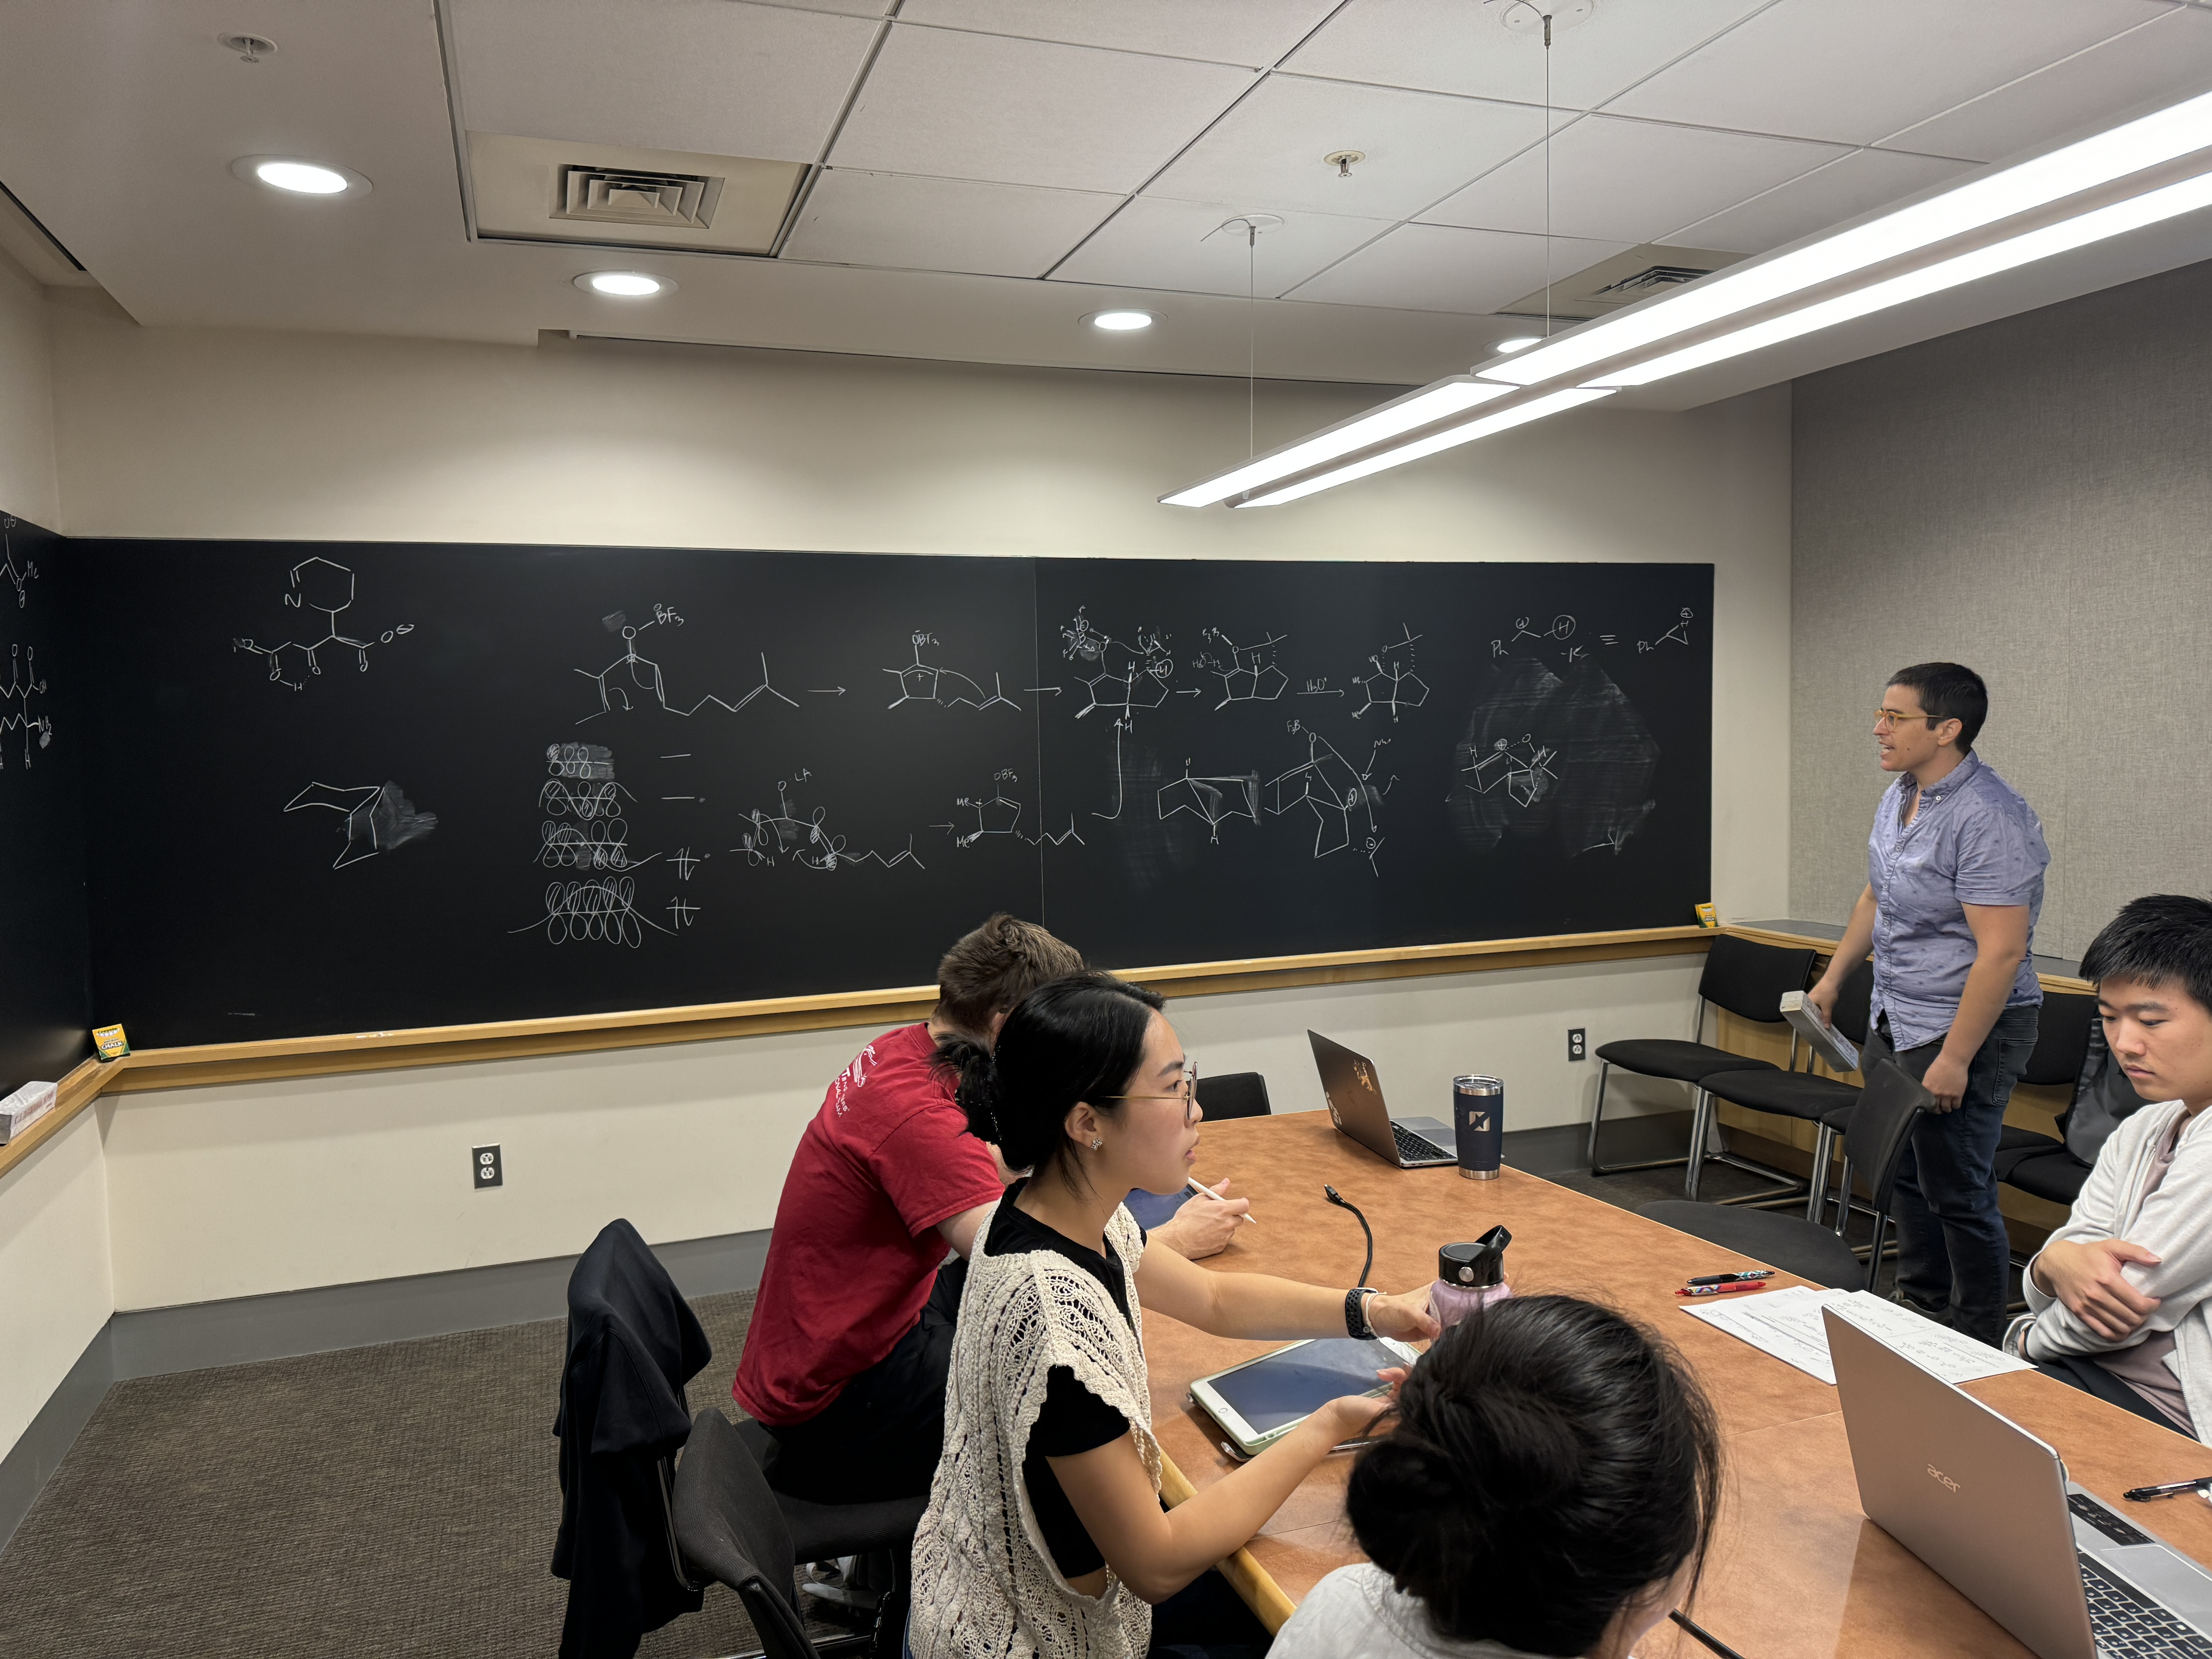
\includegraphics[width=0.8\linewidth]{WPSet1Q4S.JPG}
        \caption{Wendlandt PSet 1, Q4 solution.}
        \label{fig:WPSet1Q4S}
    \end{figure}
    \pagebreak
    \item We now begin discussing Problem 8.
    \begin{figure}[h!]
        \centering
        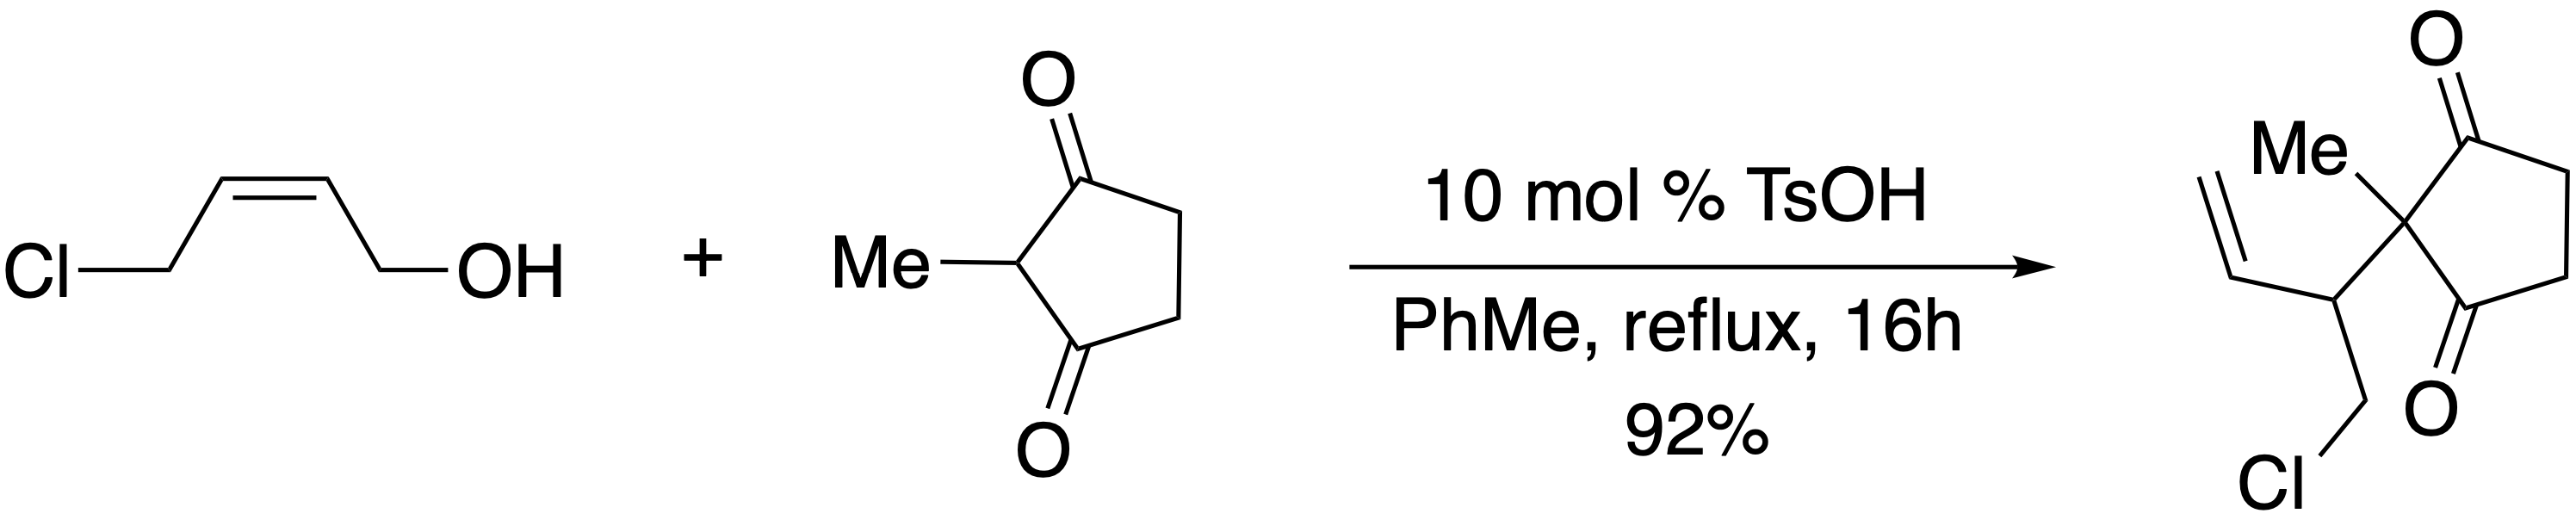
\includegraphics[width=0.6\linewidth]{WPSet1Q8.png}
        \caption{Wendlandt PSet 1, Q8.}
        \label{fig:WPSet1Q8}
    \end{figure}
    \item The thing I proposed is called an S\textsubscript{N}2' reaction, i.e., the attack of one species not on the leaving group but on the conjugated position a couple of carbons away.
    \begin{itemize}
        \item My mechanism is \emph{plausible} but not \emph{defensible}.
        \item The \ce{OH} is not the most Lewis basic species in solution.
    \end{itemize}
    \item Protonating a hemiacetal will be easier than Frank's proposition of protonating the alcohol.
    \begin{itemize}
        \item Alison proposed 1,2-addition and 1,4-addition.
    \end{itemize}
    \item We end with a \textbf{Claisen rearrangement}.
    \item You get a \emph{stabilized} enol structure. Enol is better than enolate for acidic solution.
    \item You use the nucleophilic part to rearrange the electrophilic part.
    \item Altogether, the full solution to PSet 1, Q8 is on the next page.
    \begin{figure}[h!]
        \centering
        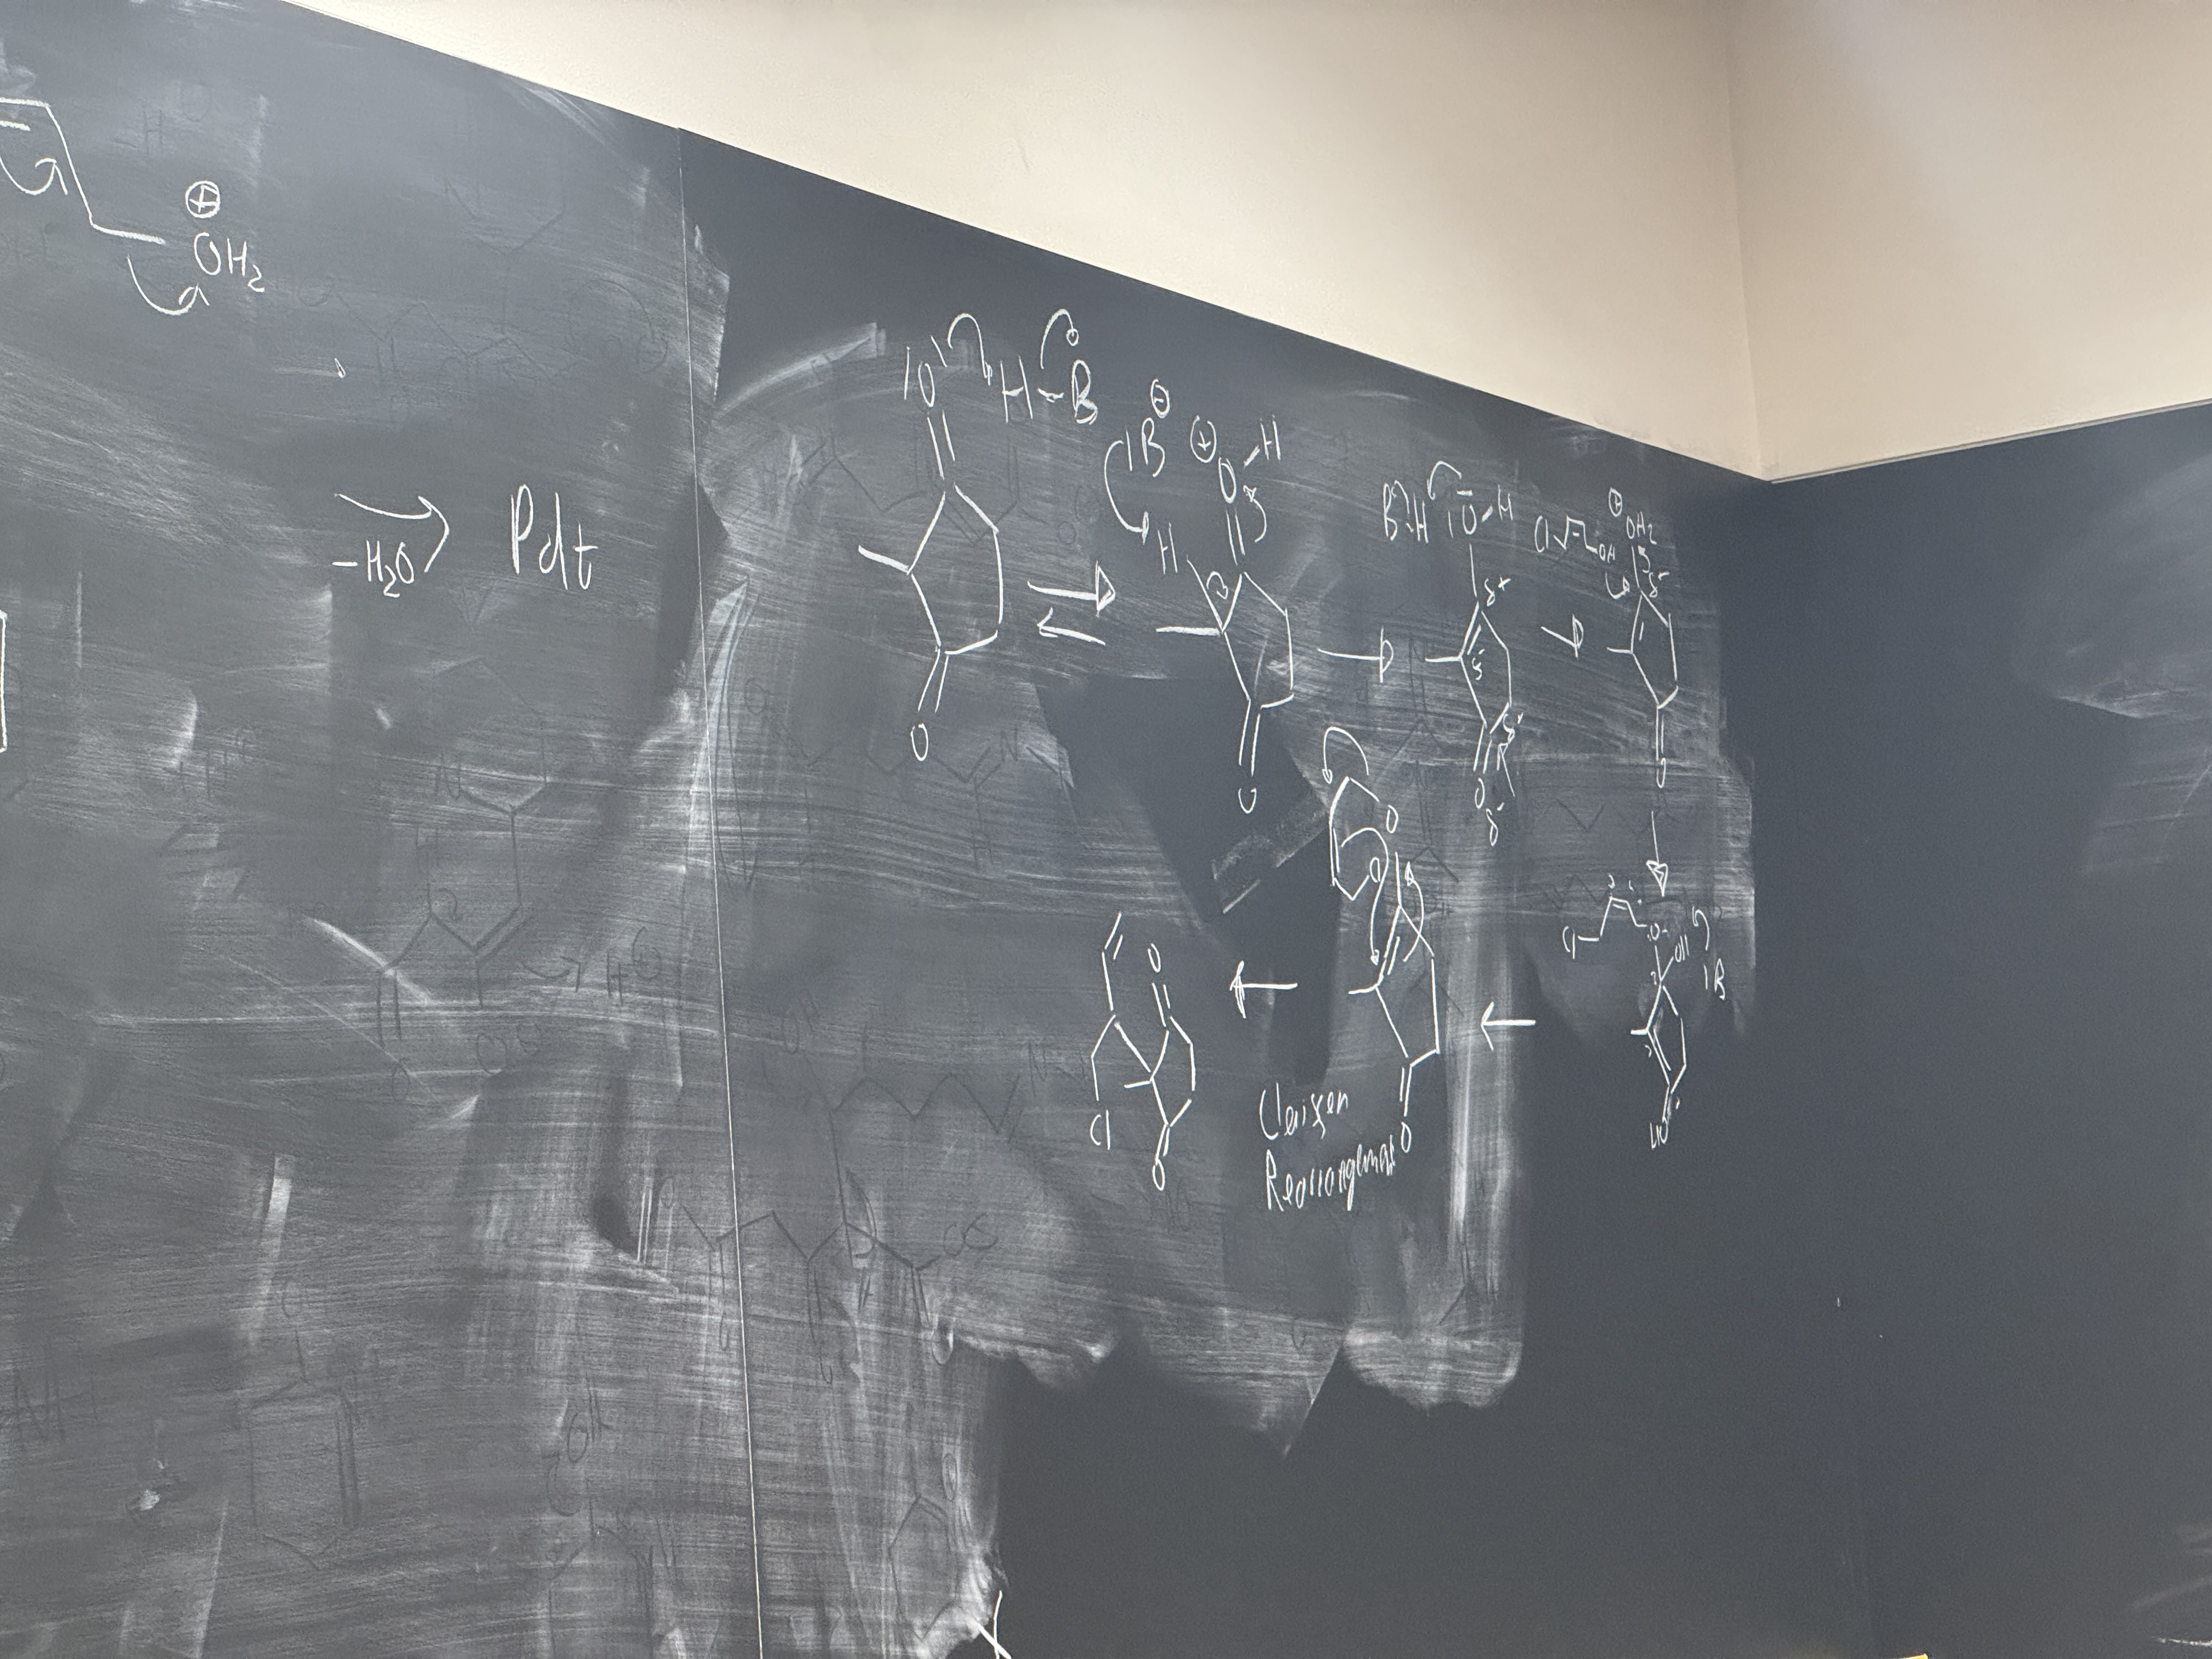
\includegraphics[width=0.8\linewidth]{WPSet1Q8S.JPG}
        \caption{Wendlandt PSet 1, Q8 solution.}
        \label{fig:WPSet1Q8S}
    \end{figure}
\end{itemize}




\end{document}